
%
% File divergences.tex


\documentclass[11pt,a4paper]{article}
\usepackage[draft]{hyperref}  % removing this line sometimes causes errors, but we should remove it still
\usepackage[hyperref]{naaclhlt2019}
\usepackage{times}
\usepackage{latexsym}

\usepackage{url}

%\aclfinalcopy % Uncomment this line for the final submission
\def\aclpaperid{287} %  Enter the acl Paper ID here

%\setlength\titlebox{5cm}
% You can expand the titlebox if you need extra space
% to show all the authors. Please do not make the titlebox
% smaller than 5cm (the original size); we will check this
% in the camera-ready version and ask you to change it back.

\usepackage[T1]{fontenc}
\usepackage{amsmath}
\usepackage{enumitem}
\usepackage{multirow}
\usepackage{tikz}
\usepackage{tikz-dependency}
\usepackage[warn]{textcomp}
\usepackage[font=small]{caption}
\usepackage{subcaption}
\usepackage{multirow}
\usepackage{etoolbox}
\usepackage{xr}
\usepackage{xfrac}
%\usepackage{listings}

\makeatletter
\renewcommand{\@BIBLABEL}{\@emptybiblabel}
\newcommand{\@emptybiblabel}[1]{}
\makeatother
\DeclareMathOperator*{\argmax}{arg\,max}

\newcommand{\com}[1]{}
\newcommand{\oa}[1]{\footnote{\color{red}OA: #1}}
\newcommand{\daniel}[1]{\footnote{\color{blue}DH: #1}}

\hyphenation{SemEval}
\hyphenation{English}
\hyphenation{French}
\hyphenation{German}


%\lstset{basicstyle=\ttfamily}


\usetikzlibrary{shapes,shapes.misc}


\title{Content Differences between Syntactic and Semantic Representations}

\author{Daniel Hershcovich$^{1,2}$ \\
  \\\And
  Omri Abend$^2$ \\
  $^1$The Edmond and Lily Safra Center for Brain Sciences \\
  $^2$School of Computer Science and Engineering \\
  Hebrew University of Jerusalem \\
  \texttt{\{danielh,oabend,arir\}@cs.huji.ac.il}
  \\\And
  Ari Rappoport$^2$
}

\date{}

\begin{document}

\maketitle

\begin{abstract}
  %1. performance gains of syntax for semantics
  %2. but, an ongoing debate
  %3. the development of "better" methods is hindered by lack of studies
  %4. we address the gap

  Syntactic analysis plays an important role in semantic parsing,
  but this role remains a topic of ongoing debate.
  The debate has been constrained by the scarcity of empirical comparative studies between syntactic and semantic schemes,
  which hinders the development of parsing methods informed by the details of target schemes and constructions.
%  as demonstrated by methods such as multi-task learning and syntactic features.
%  However, the scarcity of empirical comparative studies between syntactic and semantic schemes
  %results in existing methods being almost invariably generic,
  %  This is partly due to 
  We target this gap, and take Universal Dependencies (UD) and UCCA as a test case.
  %We emprically evaluate in what cases the two schemes converge and diverge in their content,
  After abstracting away from differences of convention or formalism,
  we find that most content divergences can ascribed to: 
  (1) UCCA's distinction between a scene and a non-scene; % as opposed to UD's POS-based distinctions;
  (2) UCCA's distinction between primary relations, secondary ones and participants; %, not accounted for by UD; 
  (3) different treatment of multi-word expressions, and
  (4) different treatment of inter-clause linkage.
  We further discuss the long tail of cases where the two schemes take markedly
  different approaches.
  Finally, we show that the proposed comparison methodology can be used
  for fine-grained evaluation of UCCA parsing.
\end{abstract}

% For camera-ready: add this to the UCCA-annotated set
% 1	unique	unique	ADJ	JJ	Degree=Pos	2	amod	_	_
% 2	gifts	gift	NOUN	NNS	Number=Plur	0	root	_	_
% 3	and	and	CCONJ	CC	_	4	cc	_	_
% 4	cards	card	NOUN	NNS	Number=Plur	2	conj	_	_


\section{Introduction}\label{sec:introduction}

  %\oa{change this to reflect the discussion as to the role of syntax}
  
  The use of syntactic parsing as a proxy for semantic structure has a long tradition in NLP.
  Indeed, syntactic parses have been leveraged by semantic parsers in a variety of ways,
  including pruning the space of possible predictions \cite{xue2004calibrating}, 
  encoding syntactic features \cite{gildea2002automatic,N15-1007,E17-1045}, 
  joint syntactic and semantic parsing \cite{surdeanu2008conll,hajivc2009conll} and
  multi-task learning \cite{strubell2018linguistically,swayamdipta2018syntactic}.
  Some syntactic representation approaches, such as CCG \cite{Steedman:00} and UD
  \citep{nivre2016universal}, directly reflect the underlying semantics, and have been used to
  transduce skeletal semantic forms using rule-based systems \cite{Basile:12,white2016universal,reddy2017universal}.
  Other works have contested the importance of syntax to semantics,
  by achieving strong performance without explicitly modeling syntax \cite{Peng-EtAl:2018:NAACL,P18-2077,P18-1192}.
  %Indeed, while some recent work contested the necessity of syntax for semantic parsing \citep{},
  %the use of syntax in semantic is still ubiqutous using methods such as multi-task learning \citep{}.
    
  Despite the centrality of this discussion, it has so far been little informed by empirical studies of
  the differences and commonalities between syntactic and semantic structures.
  Understanding such content differences can enable better ways to leverage content overlap between schemes, 
  as well as point at semantic distinctions that are unlikely to be resolved by syntax.
  A methodology for comparing syntactic and semantic treebanks can also support fine-grained error 
  analysis of semantic parsers, as demonstrated by \citet{szubert2018structured} 
  for AMR \citep{banarescu2013abstract}.
   
   This paper aims to address this gap, taking the syntactic Universal Dependencies,
  and the semantic Universal Conceptual Cognitive Annotation \cite[UCCA; ][]{abend2013universal} schemes as a test case. 
  The paper focuses on {\it content} differences, i.e., differences that cannot be resolved by simple
  conversion rules. 
  
  Selecting two relatively similar schemes, such as UD and UCCA, allows
  us to focus on content, and abstract away from differences of convention.
  One source of similarity is UD's preference of lexical heads,
  unlike other dependency schemes that prefer functional ones.
  For example, where auxiliary verbs are present (e.g., ``is eating''), UD
  marks the lexical verb ``eating'' as the head, while other schemes
  may select the inflected ``is'' as the head instead.
  While the two approaches are largely inter-translatable
  \citep{Schwartz:12}, lexical head schemes are more similar in form to semantic schemes,
   such as UCCA and broad-coverage semantic dependencies \citep{oepen2016towards},
   which facilitates their comparison.
  %Selecting more distant schemes for comparison could have potentially confounded our results.

%   Comparing relatively similar schemes therefore 
%   allows us to focus on principle differences between them, and abstract away from 
%   divergences that can be resolved straightforwardly.

  %Moreover, in order to attain cross-linguistic applicability, UD's design conventions are 
  %often not dissimilar to those made by semantic schemes. A notable example is UD's preference
  %of forming dependencies between lexical heads, rather than functional ones.
  %Moreover, UD structures have been recently transduced into skeletal semantic 
  %structures \cite[e.g.,][]{reddy2016,predpatt}, underscoring UD's conceptual similarity to semantic treebanks.
  %Since the purpose of the paper is to compare {\it content} differences, i.e., differences in the information
  %encoded by the structures, rather than their form, taking UD already cleans out much structural divergence
  %originating from differences of convention.
  

  We begin by carefully examining the structures captured by each of the annotation schemes, to find distinctions made by one but not the other. 
  We annotate 11K tokens from the English web treebank with gold standard UCCA trees, so as to have a doubly gold-annotated set.
  As UD uses bilexical trees (i.e., nodes correspond to tokens) and UCCA uses constituency-like DAGs (i.e., leaves correspond to tokens), 
  we losslessly convert the UD structures into constituency-like graphs by inserting non-terminal nodes (\S\ref{sec:methodology}). 
  
  Using the shared formalism, we align the nodes of the UD and UCCA trees, and identify which nodes have no match on the other side. 
  For the aligned nodes, we construct a ``confusion matrix'' to identify which UCCA categories are aligned with each UD relation and vice versa. 
  
%   \begin{enumerate}
%     \item 
%         Structurally convert bilexical dependency graphs into constituency-like graphs by inserting non-terminal nodes and \textit{head} edges .
%     \item 
%         Translate UD relations into UCCA edge labels by a deterministic mapping (\S\ref{sec:conversion}).
%   \end{enumerate}
  
   We find that most content differences between the schemes are due to the following
   factors (\S\ref{sec:analysis}):\daniel{add interesting example---scene-evoking noun or auxiliary verb
   \\\url{https://github.com/danielhers/UCCA_English-EWT/blob/v1-guidelines-ud/26394003.conllu} \\\url{https://github.com/danielhers/UCCA_English-EWT/blob/v1-guidelines-images/26394003.svg}}

  \begin{enumerate}[noitemsep]
      \item UCCA's central distinction is whether a phrase evoke a Scene (event),
        whereas UD's is based on part of speech. % (\S\ref{sec:scenes}).
      \item UCCA distinguishes Participants and secondary relations, such
        as  from adjuncts, as opposed to UD's core/non-core distinction. % (\S\ref{sec:arguments}).
        \daniel{primary, secondary and participants}
      \item Multi-word expressions are handled differently,
        where UCCA has a stronger tendency to group multiple 
        words into a single unit. % (\S\ref{sec:mwe}).
      \item UCCA conflates several syntactic realizations of inter-clause linkage that UD sets apart,
        treating them as one semantic phenomenon. % (\S\ref{sec:linkage}).
        \daniel{handled differently... on the other hand, distinguishes between linkage types}
   \end{enumerate}
    
  \oa{what was wrong with what I wrote before?}
    
   Other divergences stem from a different treatment of coordination, apposition and copulas (\S\ref{sec:misc}).
  
  %  We further extend the structural converter built as part of our analysis to
  %  get a full labeled converter (\S\ref{sec:conversion}),
  %  and use it to generate silver standard training data for a UCCA parser (\S\ref{sec:silver}).
  %  As another use-case for our converter to support parsing,

  To demonstrate the utility of our comparison methodology,
  we perform fine-grained error analysis on UCCA parsing results
  according to UD relations (\S\ref{sec:fine_grained}).
  We show that this analysis both highlights challenges for existing UCCA parsing technology,
  as well suggests where the parsers may benefit from relying on the syntactic structure more directly.

%  The motivation for parsing into semantic structural representation is that it can be used more readily
%  by semantic applications to reason about the processed utterance and manipulate it to find the required
%  result.
%  For example, in machine translation, a common model is the Vauquois Pyramid 
%  \cite{vauquois1968survey},
%  according to which translation between languages will become easier and more direct as we use
%  a more semantic representation for the source and target languages,
%  ignoring language-specific distinctions and capturing only what is preserved in translation.
%  Parsing the source language and generating the target language, on the other hand, becomes more
%  difficult as the representation becomes more semantic.

\daniel{We should cite \newcite{abend2017state}}
%  Semantic representation schemes have seen major progress in recent years \cite{abend2017state}.
%  At the same time, semantic considerations are taken into account in the design of syntactic annotation schemes
%  \cite{przepiorkowski2018arguments}.

%  \begin{itemize}
%    \item Evaluation metric,
%    \item Amount of training data,
%    \item Maturity of technology dedicated to the scheme,
%    \item Learnability of the scheme.
%  \end{itemize}
%  Learnability, in turn, is affected by
%  \begin{itemize}
%    \item Formal annotation choices \cite{Schwartz:12},
%    \item Actual content that the scheme attempts to capture.
%  \end{itemize}

%Different schemes capture different content.
%For example, dependencies are ambiguous as to the arguments of conjoined verbs:
%``the store buys and sells cameras'' and ``she was reading or watching a movie''
%are analyzed similarly, even though in the first sentence ``cameras'' is an argument
%of both ``buys'' and ``sells'', and in the second sentence ``movie'' is only an argument
%of ``watching''.
%The UCCA representation does make this distinction, as Figure~\ref{fig:conjoined_verbs} shows.
%
%\begin{figure}[!ht]
%  \centering
%    \begin{tikzpicture}[level distance=12mm, ->,
%        level 1/.style={sibling distance=21mm},
%        level 2/.style={sibling distance=11mm},
%        every circle node/.append style={fill=black}]
%      \tikzstyle{word} = [font=\rmfamily,color=black]
%      \node (ROOT) [circle] {}
%        child {node [circle] {}
%        {
%          child {node (She) [word] {She} edge from parent node[above] {\scriptsize $A$}}
%          child {node (was) [word] {was} edge from parent node[left] {\scriptsize $F$}}
%          child {node [word] {reading} edge from parent node[below] {\scriptsize $P$}}
%        } edge from parent node[left] {\scriptsize $H$} }
%        child {{}
%        {
%          child {node (or) [word] {or} edge from parent [draw=none]}
%        } edge from parent [draw=none]}
%        child {node (watchingamovie) [circle] {}
%        {
%          child {node [word] {watching} edge from parent node[left] {\scriptsize $P$}}
%          child {node [circle] {}
%          {
%            child {node [word] {a} edge from parent node[left] {\scriptsize $E$}}
%            child {node [word] {movie} edge from parent node[right] {\scriptsize $C$}}
%          } edge from parent node[above] {\scriptsize $A$} }
%        } edge from parent node[right] {\scriptsize $H$} }
%        ;
%      \draw[dashed,->,bend right=20] (watchingamovie) to node [above] {\scriptsize $A$} (She);
%      \draw[dashed,->,bend right=10] (watchingamovie) to node [above] {\scriptsize $F$} (was);
%      \draw(ROOT) to node [right] {\scriptsize $L$} (or);
%    \end{tikzpicture}
%\caption{Coordinated predicates in UCCA.
%\label{fig:conjoined_verbs}}
%\end{figure}

%Apart from the set of distinctions each scheme makes,
%an important driver of the difference in scores is the proportion of each constructions
%in the evaluation.
%This implicitly determines what the scheme focuses on and what parser developers
%will spend a larger effort improving.
%
%For example, punctuation takes up 11.4\% of the edges in the English EWT UD treebank,
%and parsers typically achieve more than 90\% LAS F1 on punctuation.
%In UCCA, punctuation is excluded from the evaluation completely.
%
%A multi-word named entity is represented in UD by a \texttt{flat} arc between
%each pair of consecutive words in the entity mention.
%In UCCA, a named entity is represented as one unanalyzable unit, and analyzing it
%incorrectly results in an incorrect edge with no partial credit.


%%%%%%%%%%%%%%%%%%%%%%%%%%%%%%%%%%%%%%%%%%%%%%%%%%%%%%%%%%%%%%%%%%%%%%%%%%%%%%%%%

\section{Representations}\label{sec:representations}

  The conceptual and formal similarity between UD and UCCA can be traced back
  to their shared design principles.
  Both schemes are designed to be applicable across languages and domains, 
  to support rapid annotation and to be suitable for downstream language understanding
  applications. This section provides a brief introduction to each of the schemes, whereas
  the next sections discuss their content in further
  detail.\footnote{See Supplementary Material for a definition of each category in both schemes.}
  


\paragraph{UCCA}\label{sec:ucca}
  \citep[Universal Cognitive Conceptual Annotation;][]{abend2013universal} is a semantic annotation scheme rooted in typological 
  and cognitive linguistic theory.
  It aims to represent the main semantic phenomena in the text, abstracting away from syntactic forms.
  UCCA has been shown to be preserved remarkably well across translations \citep{sulem2015conceptual} and has also been applied to
  improve text simplification \citep{sulem2018simple} used text-to-text generation evaluation \citep{birch2016hume,choshen2018usim,sulem2018samsa}.

  Formally, UCCA structures are directed acyclic graphs whose nodes (or {\it units}) correspond either to the leaves of the graph %(including the words of the text)%
  or to several elements viewed as a single entity according to some semantic or cognitive consideration.
  Edges are labeled, indicating the role of a child in the relation the parent represents.
  A {\it Scene} is UCCA's notion of an event or a frame, and is a description of a movement, an action or a state which persists in time. 
  Every Scene contains one main relation, which can be either a Process or a State. 
  Scenes may contain any number of Participants, a category which also includes abstract participants and locations.
  They may also contain secondary relations (Adverbials), which cover semantic distinctions such as manner, modality and aspect,
  and temporal relations (Time).

  Scenes may be linked to one another in several ways. First, a Scene can provide additional information about some entity,
  in which case it will be marked as an Elaborator. This often occurs in the case of participles or relative clauses.
  For example, ``(child) who went to school'' is an Elaborator (Scene)
  in ``The child who went to school is John''.
  A Scene may also be a Participant in another Scene. For example, ``John went to school'' in the sentence: ``He said John went to school''. 
  In other cases, Scenes are annotated as Parallel Scenes (H), which are flat structures and may include a Linker (L), 
  as in:  ``When$_L$ [he arrives]$_H$, [he will call them]$_H$''.

  With respect to non-Scene units, the category Center denotes their semantic head, which determine their type. 
  Other elements in non-Scene units include Quantifiers (such as ``{\bf dozens} of people''), Connectors (mostly
  coordinating conjunctions, and Relators, that in English correspond to prepositions.
  Other modifiers to the Center are marked as Elaborators.
  
  UCCA distinguishes \textit{primary} edges, corresponding 
  to explicit relations, from \textit{remote} edges (appear dashed in
  Figure~\ref{fig:example_ucca}) that allow for a unit to participate
  in several super-ordinate relations.
  Primary edges form a tree, whereas remote edges enable reentrancy, forming a DAG.
  %Table~\ref{} gives a short description of each UCCA category.  % supp. material (footnote above)




  %UCCA's foundational layer \cite{abend2013universal} (UCCA, for brevity) 
  %is a coarse-grained semantic annotation scheme, which focuses
  %on predicate argument structures, the linkage between them, and the notion of a semantic head.
  %UCCA structures as directed acyclic graphs (DAGs), where terminal (childless) nodes
  %correspond to the text tokens, and non-terminal nodes to semantic units that participate
  %in some super-ordinate relation.
  

  %Nodes and edges belong to one of several \textit{layers}, each corresponding
  %to a ``module'' of semantic distinctions.
  %UCCA's \textit{foundational layer} (the only layer for which annotated data exists)
  %mostly covers predicate-argument structure, semantic heads and inter-Scene relations.
  
  



\begin{figure}[!ht]
  \centering
    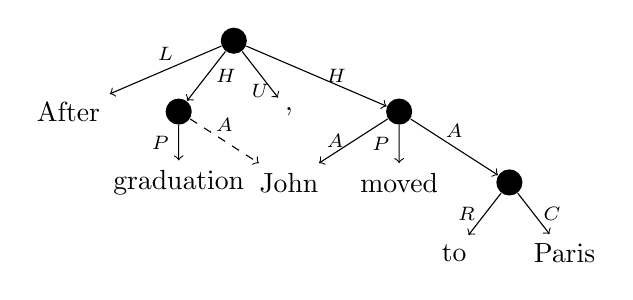
\begin{tikzpicture}[level distance=9mm, sibling distance=14mm, ->,
        every circle node/.append style={fill=black}]
      \tikzstyle{word} = [font=\rmfamily,color=black]
      \node (ROOT) [circle] {}
        child {node (After) [word] {After} edge from parent node[above] {\scriptsize $L$}}
        child {node (graduation) [circle] {}
        {
          child {node [word] {graduation} edge from parent node[left] {\scriptsize $P$}}
        } edge from parent node[right] {\scriptsize $H$} }
        child {node [word] {,} edge from parent node[below] {\scriptsize $U$}}
        child {node (moved) [circle] {}
        {
          child {node (John) [word] {John} edge from parent node[left] {\scriptsize $A$}}
          child {node [word] {moved} edge from parent node[left] {\scriptsize $P$}}
          child {node [circle] {}
          {
            child {node [word] {to} edge from parent node[left] {\scriptsize $R$}}
            child {node [word] {Paris} edge from parent node[right] {\scriptsize $C$}}
          } edge from parent node[above] {\scriptsize $A$} }
        } edge from parent node[right] {\scriptsize $H$} }
        ;
      \draw[dashed,->] (graduation) to node [above] {\scriptsize $A$} (John);
    \end{tikzpicture}
\caption{\label{fig:example_ucca}
 Example UCCA graph. Dashed: a remote edge.
%  Pre-terminal nodes and edges are omitted for brevity.
  }
\end{figure}

%%%%%%%%%%%%%%%%%%%%%%%%%%%%%%%%%%%%%%%%%%%%%%%%%%%%%%%%%%%%%%%%
\paragraph{Universal Dependencies.}\label{sec:ud}
UD \cite{nivre2016universal} has quickly become
the dominant dependency scheme for
syntactic  annotation in many languages,
aiming for cross-linguistically consistent and coarse-grained treebank
annotation. Formally, UD uses bilexical trees, with edge labels 
representing syntactic relations between words.
Figure~\ref{fig:original_example_ud} shows an example UD tree.
%and Table \ref{} gives a short description of each UD category.  % supp. material (footnote above)
Henceforth in this paper, UD relation labels are written in \texttt{typewriter} font.

\begin{figure}[!ht]

\fbox{\begin{subfigure}{0.47\textwidth}
  \centering
    \begin{dependency}[text only label, label style={above,font=\tt}, font=\small]
    \begin{deptext}[column sep=.8em,ampersand replacement=\^]
    After \^ graduation \^ , \^ John \^ moved \^ to \^ Paris \\
    \end{deptext}
        \depedge[edge unit distance=1ex]{2}{1}{case}
        \depedge[edge unit distance=1ex]{4}{3}{punct}
        \depedge[edge unit distance=1ex]{5}{4}{nsubj}
        \depedge[edge unit distance=1ex, edge end x offset=-2pt]{2}{5}{obl}
        \depedge[edge unit distance=1ex]{7}{6}{case}
        \deproot[edge unit distance=1.5ex]{5}{root}
        \depedge[edge unit distance=1.5ex]{5}{7}{obl}
    \end{dependency}
  \caption{UD \label{fig:original_example_ud}}
\end{subfigure}}

\fbox{\begin{subfigure}{0.47\textwidth}
  \centering
  \scalebox{.95}{
  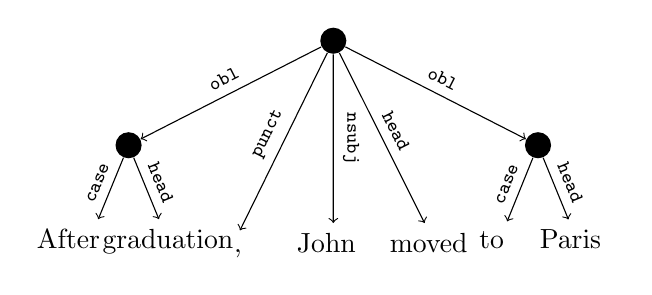
\begin{tikzpicture}[level distance=15mm, ->,
      every node/.append style={sloped,anchor=south,auto=false,font=\scriptsize\tt},
      level 1/.style={sibling distance=13mm},
      level 2/.style={sibling distance=1cm}]
    \tikzstyle{word} = [font=\rmfamily,color=black]
    \node (ROOT) [fill=black,circle] {}
      child {node (after) [fill=black,circle] {}
      {
        child {node [word] {After{\color{white}g}\quad\quad} edge from parent node {case}}
        child {node [word] {\quad graduation\quad\quad} edge from parent node {head}}
      } edge from parent node {obl}}
      child {node {}
      {
        child {node [word] (comma) {\quad,{\color{white}g}} edge from parent [draw=none]}
      } edge from parent [draw=none]}
      child {node {}
      {
        child {node [word] (John) {John{\color{white}g}} edge from parent [draw=none]}
      } edge from parent [draw=none]}
      child {node {}
      {
        child {node [word] (moved) {moved{\color{white}g}} edge from parent [draw=none]}
      } edge from parent [draw=none]}
      child {node (to) [fill=black,circle] {}
      {
          child {node [word] {to{\color{white}g}} edge from parent node {case}}
          child {node [word] {Paris{\color{white}g}} edge from parent node {head}}
      } edge from parent node {obl}}
      ;
      \draw (ROOT) to node {punct} (comma);
      \draw (ROOT) to node {nsubj} (John);
      \draw (ROOT) to node {head} (moved);
  \end{tikzpicture}}
  \captionof{figure}{UD}\label{fig:converted_example_ud}
\end{subfigure}}

\caption{Figure \ref{fig:original_example_ud} presents a UD tree.
  Edge labels express syntactic relations.
Figure~\ref{fig:converted_example_ud} presents a converted UD graph.
%(with pre-terminals omitted: each terminal drawn in place of its parent).
Intermediate non-terminals and \textit{head} edges are introduced.
%While converted UD graphs form trees, enhanced++ UD graphs may not.
}\label{fig:ud_examples}
\end{figure}


%%%%%%%%%%%%%%%%%%%%%%%%%%%%%%%%%%%%%%%%%%%%%%%%%%%%%%%%%%%%%%%%%%%%%%%%%%%%%%%%%%%%%%%%%%%%%%5
\section{Shared Gold Standard Corpus}\label{sec:shared}

We annotate 163 English passages, containing 804 sentences
from the \textit{reviews} section of the 
English Web Treebank \cite[EWT; ][]{bies2012english}.
The sentences are annotated by two UCCA annotators
according to v2.0 of the UCCA
guidelines\footnote{{\scriptsize \url{github.com/UniversalConceptualCognitiveAnnotation/docs}}}
and cross-reviewed.\footnote{The data will be released upon publication.}
As these sentences are included in the Universal Dependencies 
English\_EWT treebank, we have both gold-standard UCCA and UD for them. 
We refer to this set as \textit{shared} henceforth.

The data contains 11,103 tokens, constituting 4\% of the full UD English\_EWT treebank,
and 20\% of its \textit{reviews} section.
%(see Table~\ref{tab:corpora}).
Of the UCCA-annotated sentences, 622 belong to the UD training set,
192 to the development set and 153 to the test set.\daniel{Add inter-annotator agreement}


%%%%%%%%%%%%%%%%%%%%%%%%%%%%%%%%%%%%%%%%%%%%%%%%%%%%%%%%%%%%%%%%%%%%%%%%%%%%%%%%%%%%%%%%%%%%%%5
\section{Comparison Methodology}\label{sec:methodology}

To facilitate comparison between UCCA and UD,
we first assimilate the graphs by abstracting away from formalism differences,
obtaining a similar graph format for both schemes,
over the tokens of the sentence.
We then match pairs of nodes in the converted UD and UCCA trees
if they share the same set of terminals in their yields.\oa{maybe explain about unary expansions?} % (\S\ref{sec:analysis}).

One obvious difference is that UD annotates bi-lexical dependency graphs,
while UCCA graphs contain non-terminal nodes.
To reach a common format, we use the unified DAG converter by
\citet{hershcovich2018multitask,hershcovich2018universal},\footnote{\url{http://github.com/huji-nlp/semstr}}
outlined in \S\ref{sec:conversion}.
Then, in \S\ref{sec:local}, we describe a number of extensions
to the converter, which abstract away from further non-content differences between the converted
UD and UCCA graphs.





%<<<<<<< HEAD
%\cite{SCHUSTER16.779} representing case information, elided predicates,
%and shared argumenthood due to coordination, control, raising and relative clauses.
%They provide richer information to downstream semantic applications,
%making UD better suited for text understanding.
%Enhanced UD has a more restricted notion of shared arguments than UCCA's,
%which includes the class of implicit arguments termed {\it Constructional
%Null Instantiation} in FrameNet. For instance, in ``to win, you have to find the key'',
%UCCA would add a remote 
%=======
%as part of the dependency graph,
%representing elided predicates,
%and shared arguments due to coordination, control, raising and relative clauses.
% case information
%They provide richer information to downstream semantic applications,
%making UD better suited for text understanding.
%Enhanced UD has a more restricted notion of shared arguments than UCCA's.
%\daniel{reviews-220214-0002: ``First of all, if you call for an appointment they won't tell you to call back a month later so you can then make one'',
%weblog-blogspot.com\_rigorousintuition\_20060511134300\_ENG\_20060511\_134300-0106:
%``The Pentagon is bypassing official US intelligence channels and turning to a dangerous and unruly cast of characters in order to create strife in Iran in preparation for any possible attack, former and current intelligence officials say...''.}





\subsection{Basic Conversion}\label{sec:conversion}

Figure~\ref{fig:converted_example_ud} presents an example UD tree conversion.
Given a UD tree, the converter adds a pre-terminal for each token,
and attaches the pre-terminals according to the original dependency edges:
traversing the tree from the root down, for each head token it creates a non-terminal
parent with the edge label {\it head}, and adds the node's dependents as children of 
the created non-terminal node.
%Any \textit{enhanced}
%heads beyond the normal head of a node are converted to remote edges in the unified DAG format.
In the conversion process, any language-specific relation subtypes are stripped,
leaving only the universal relations.
For example, the language-specific label for definite artciles
\texttt{det:def} is replaced by the universal relation \texttt{det}.

In the UCCA format, edges are labeled (but not nodes),
and are divided into \textit{primary} and \textit{remote} edges
(e.g., the dashed edge in Figure~\ref{fig:example_ucca}),
where the primary edges form a tree (all nodes have at most one primary parent,
and the root has none).
Remote edges enable reentrancy, and thus together with primary edges form a DAG.
UD includes \textit{enhanced dependencies}\footnote{\url{http://universaldependencies.org/u/overview/enhanced-syntax.html}}
\cite{SCHUSTER16.779}, which form (bi-lexical) DAG structures, representing phenomena
such as predicate ellipsis (e.g., gapping),
and shared arguments due to coordination, control, raising and relative clauses.

UCCA is more inclusive in its use of remote edges, and accounts for 
the entire class of implicit arguments termed {\it Constructional Null Instantiation} in FrameNet \citep{Ruppenhofer:16}.
For example, UCCA adds a remote edge to mark the shared argumenthood of ``bypassing'' and
``create'' in ``The Pentagon is bypassing official US intelligence channels ... in order to create strife ...'' (from EWT). 
Another example is ``... if you call for an appointment they won't tell you to call back a month later so you can then make one'',
where UCCA will use a remote edge to indicate that ``one'' refers to appointment.
Both cases are not covered by enhanced UD.

In order to facilitate comparison, we remove remote edges and enhanced dependencies in the conversion process.
We thus compare UD and UCCA trees. We defer a more complete comparison of UCCA and enhanced UD to future work.


%In the UCCA format, edges are labeled (but not nodes),
%and are divided into \textit{primary} and \textit{remote} edges,
%where the primary edges form a tree (all nodes have at most one primary parent,
%and the root has none). Remote edges enable reentrancy, and thus together with primary edges
%form a DAG. In order to facilitate comparison, and as UD does not support reentrancy,\footnote{Reentracy is supported by enhanced UD \cite{SCHUSTER16.779}.} We remove remote edges in the conversion process.
%Figure~\ref{fig:converted_example_ud} shows an example for a converted graph.



%\oa{move this paragraph some place else}
%  UCCA graphs are converted into trees by removing ``remote edges''.
%  Remote edges in UCCA encode shared argumenthood by assigning multiple parents to the same node. Such phenomena are largely ignored in UD, %which uses trees. See \S\ref{sec:analysis}.



\subsection{Extensions to the Converter}\label{sec:local}

We extend the converter to remove further non-content differences.

\paragraph{Unanalyzable units.}
Unanalyzable phrases are represented in UCCA as a single unit covering multiple terminals.
As for multi-word expressions (MWEs) in UD, each word after the first is attached to the previous word,
with the \texttt{flat}, \texttt{fixed} or \texttt{goeswith} relations
(depending on whether the phrase is a name or a title, a fixed grammaticalized MWE
or whether it is one word split by error).
During conversion, we remove edges of both relations and group the corresponding terminals to one unit.
%Multi-word expressions also include compounds, discussed in \S\ref{sec:mwe}.

\paragraph{Promotion of conjunctions.}
The basic conversion protocol generally attaches low so as to preserve terminal yields:
the set of terminals spanned by a non-terminal is the same
as the original dependency yield of its head terminal
(e.g., in Figure~\ref{fig:converted_example_ud}, the yield of the non-terminal
headed by ``graduation'' is ``After graduation'', the same as the yield of ``graduation''
in Figure~\ref{fig:original_example_ud}).
%selecting for each terminal $t$ the lowest non-terminal of which $t$
%is the head terminal to be its parent.

Since UD attaches subordinating and coordinating conjunctions to the following conjunct,
this results in them being positioned as part
of the conjuncts they relate (e.g., ``and'' will be included in the second conjunct in ``John and Mary''; 
``after'' will be included in the first conjunct in ``After arriving home, John went to sleep'').
In contrast, UCCA places conjunctions as siblings to their conjuncts (e.g., ``[John] [and] [Mary]'' or
``[After] [arriving home], [John went to sleep''). 

To abstract away from these convention differences,
we extend the conversion protocol to place 
the dependents of coordinating and subordinating conjunctions 
(i.e., \texttt{cc}-labeled units, and \texttt{mark}-labeled units with an \texttt{advcl} head such 
as ``when'', ``if'', ``after'') as siblings to their conjuncts.
%as there is a systematic mapping between the UCCA and UD guidelines
%and it is different from the default low-attaching behavior.


%Some conjunctions are placed in UCCA as siblings of the units they link,
%while in UD they are dependents of the dependent unit. For instance, coordinating
%conjunctions (e.g., ``and'' in ``John and Mary'') are in UCCA siblings of the conjuncts 
%Selecting a forward-attaching behavior instead:
%\begin{itemize}
%  \item Conjunctions (\texttt{cc} in UD) attach to the following
%  conjuncts (word with an incoming \texttt{conj} relation).
%  \item \texttt{mark} is attached to the following \texttt{advcl}.
%\end{itemize}
%These rules are applied to the bilexical graph after the conversion process.




%%%%%%%%%%%%%%%%%%%%%%%%%%%%%%%%%%%%%%%%%%%%%%%%%%%%%%%%%%%%%%%%%%%%%%%%%%%%%%%
\section{Analysis of Divergences}\label{sec:analysis}

We turn to discussing the content differences between UCCA and UD.
%as quantified in a \textit{confusion matrix} between the schemes (\S\ref{sec:confusion}).


\begin{table}[t]
\centering
\scriptsize
\setlength\tabcolsep{2pt}
\begin{tabular}{l|cccccccccccc|c}
 & \bf \rotatebox{90}{Participant (A)} & \bf \rotatebox{90}{Center (C)}
 & \bf \rotatebox{90}{Adverbial (D)} & \bf \rotatebox{90}{Elaborator (E)}
 & \bf \rotatebox{90}{Function (F)} & \bf \rotatebox{90}{Ground (G)}
 & \bf \rotatebox{90}{ Parallel Scene (H)} & \bf \rotatebox{90}{Linker (L)}
 & \bf \rotatebox{90}{Connector (N)} & \bf \rotatebox{90}{Process (P)}
 & \bf \rotatebox{90}{Relator (R)} & \bf \rotatebox{90}{State (S)}
 & \rotatebox{90}{{\sc NoMatch}} \\
\hline
\bf \tt \tiny acl & 8 & 0 & 0 & 101 & 2 & 0 & 15 & 0 & 0 & 0 & 0 & 1 & 49 \\
\bf \tt \tiny advcl & 2 & 2 & 0 & 0 & 0 & 0 & 103 & 1 & 0 & 4 & 0 & 0 & 97 \\
\bf \tt \tiny advmod & 61 & 9 & 524 & 53 & 12 & 33 & 3 & 61 & 0 & 2 & 6 & 5 & 71 \\
\bf \tt \tiny amod & 1 & 33 & 106 & 218 & 2 & 0 & 7 & 0 & 0 & 3 & 0 & 97 & 61 \\
\bf \tt \tiny appos & 1 & 10 & 1 & 8 & 0 & 0 & 5 & 0 & 0 & 0 & 0 & 4 & 10 \\
\bf \tt \tiny aux & 0 & 0 & 96 & 0 & 285 & 0 & 0 & 0 & 0 & 0 & 0 & 0 & 2 \\
\bf \tt \tiny case & 1 & 5 & 2 & 15 & 34 & 0 & 0 & 48 & 6 & 1 & 489 & 50 & 75 \\
\bf \tt \tiny cc & 0 & 0 & 1 & 1 & 0 & 0 & 0 & 305 & 71 & 0 & 1 & 0 & 11 \\
\bf \tt \tiny ccomp & 78 & 0 & 0 & 0 & 0 & 0 & 8 & 0 & 0 & 0 & 0 & 1 & 41 \\
\bf \tt \tiny compound & 23 & 24 & 11 & 174 & 2 & 0 & 0 & 0 & 0 & 1 & 1 & 3 & 167 \\
\bf \tt \tiny conj & 2 & 88 & 1 & 0 & 0 & 0 & 265 & 0 & 0 & 2 & 0 & 3 & 90 \\
\bf \tt \tiny cop & 0 & 0 & 0 & 0 & 333 & 0 & 0 & 0 & 0 & 3 & 1 & 24 & 3 \\
\bf \tt \tiny csubj & 2 & 0 & 0 & 0 & 0 & 0 & 0 & 0 & 0 & 0 & 0 & 0 & 8 \\
\bf \tt \tiny det & 2 & 1 & 23 & 778 & 1 & 1 & 0 & 0 & 0 & 0 & 2 & 0 & 26 \\
\bf \tt \tiny discourse & 0 & 1 & 0 & 0 & 1 & 6 & 13 & 3 & 0 & 0 & 0 & 1 & 1 \\
\bf \tt \tiny expl & 0 & 0 & 0 & 0 & 22 & 0 & 0 & 0 & 0 & 0 & 0 & 0 & 2 \\
\bf \tt \tiny iobj & 19 & 0 & 0 & 0 & 0 & 0 & 0 & 0 & 0 & 0 & 0 & 0 & 0 \\
\bf \tt \tiny list & 0 & 2 & 0 & 0 & 0 & 0 & 8 & 0 & 0 & 0 & 0 & 0 & 2 \\
\bf \tt \tiny mark & 0 & 2 & 4 & 0 & 161 & 1 & 0 & 159 & 1 & 0 & 53 & 1 & 18 \\
\bf \tt \tiny nmod & 100 & 1 & 5 & 231 & 0 & 0 & 6 & 0 & 0 & 0 & 0 & 3 & 112 \\
\bf \tt \tiny nsubj & 993 & 0 & 0 & 0 & 14 & 0 & 2 & 9 & 0 & 3 & 24 & 1 & 37 \\
\bf \tt \tiny nummod & 4 & 7 & 3 & 53 & 0 & 0 & 3 & 0 & 0 & 0 & 0 & 0 & 24 \\
\bf \tt \tiny obj & 439 & 7 & 10 & 1 & 1 & 0 & 1 & 1 & 0 & 8 & 6 & 0 & 92 \\
\bf \tt \tiny obl & 247 & 1 & 92 & 8 & 2 & 4 & 4 & 4 & 0 & 0 & 2 & 0 & 132 \\
\bf \tt \tiny parataxis & 1 & 0 & 0 & 1 & 0 & 2 & 79 & 0 & 0 & 1 & 0 & 2 & 39 \\
\bf \tt \tiny vocative & 9 & 0 & 0 & 0 & 0 & 3 & 0 & 0 & 0 & 0 & 0 & 0 & 0 \\
\bf \tt \tiny xcomp & 44 & 1 & 2 & 2 & 0 & 0 & 1 & 0 & 0 & 5 & 0 & 7 & 116 \\
\hline
head & 124 & 1,402 & 157 & 51 & 91 & 18 & 652 & 2 & 1 & 961 & 9 & 353 & 526 \\
{\sc NoMatch} & 330 & 172 & 53 & 73 & 6 & 5 & 466 & 29 & 0 & 141 & 7 & 98
\end{tabular}
\caption{UD-UCCA confusion matrix calculated from EWT
gold-standard annotations (\S\ref{sec:shared}),
after converting UD to the unified DAG format,
by comparing incoming edge labels for units with the same terminal yields.
The last column (row), labeled {\sc NoMatch}, shows the number of edges of each UD (UCCA) category
that do not match any UCCA (UD) unit.\daniel{Update to include Time and Quanitifer}
\label{tab:confusion_matrix}}
\end{table}

\subsection{Confusion Matrix}\label{sec:confusion}

%Using the standard UCCA evaluation
%script,\footnote{\url{http://github.com/huji-nlp/ucca/blob/master/scripts/evaluate_standard.py}}
Table~\ref{tab:confusion_matrix} presents the confusion matrix between the edge tags in converted UD trees
and the annotated UCCA graphs.
%Using the standard UCCA evaluation
%script,\footnote{\url{http://github.com/huji-nlp/ucca/blob/master/scripts/evaluate_standard.py}}
%we create a confusion matrix between the edge tags in converted UD trees
%and the annotated UCCA graphs (see Table~\ref{tab:confusion_matrix}).
In case of multiple units with the same terminal yield (i.e., any unit with a single non-remote child),
we take the top category only to avoid double-counting.
We perform this analysis on gold-standard UD and UCCA from the shared EWT corpus
(see \S\ref{sec:shared}),
after conversion to the unified DAG format.
Excluding punctuation, this results in 12893 yields in UCCA and
13294 in UD.
Of these, 11541 are common, meaning that an oracle UCCA ``parser'' developed this way
would get a very high F1 score
of 88.1\% if it had the gold UCCA label for every edge on conversion.

Examining the {\it head} row in Table \ref{tab:confusion_matrix} allows
us to contrast UCCA's and UD's notions of a head. 
{\it head}-labeled units cover units that have at least
one dependent in UD (technically, they are non-terminals added by the converter).
%About 70\% of them correspond to UCCA Processes, States,  Parallel Scenes or Centers,
%which are UCCA's notions of semantic heads.
77.5\% correspond to UCCA Processes, States, Linked Scenes or Centers,
which are UCCA's notions of semantic heads.
12.1\% of the {\it head} units are left unmatched, mostly due to MWEs analyzed in
UD but not in UCCA (\S\ref{sec:mwe}).
Another source of unmatched units is inter-scene linkage, which tends to be flatter in
UCCA (see \S\ref{sec:linkage}).
The remaining cases (10.4\%) are mostly due to a head swap (e.g., ``\textit{all} of Dallas'', where \textit{all} 
is an Elaborator of ``Dallas'' in UCCA, but the syntactic head in UD).

In the following subsections, we review the main content differences between the schemes,
as reflected in the confusion matrix, and categorize them according to the UD relations
involved.

%categorize UD relations according to their
%treatment in UCCA, focusing of the main content differences between the schemes.

\subsection{Scenes vs. Non-scenes}\label{sec:scenes}

UCCA distinguishes between Scenes and Non-scenes. 
This distinction cuts across UD categories,
as a Scene can be evoked by a verb, an eventive or stative
noun (``negotiation'', ``fatigue''),
an adjective or even a preposition (``this is \textit{for} John'').

\begin{description}
    \item[Core Arguments (\texttt{iobj}, \texttt{nsubj}, and \texttt{obj}).] 
      Core syntactic arguments are usually UCCA Participants (e.g., ``\textit{Wine} was excellent'').
      However, when describing a scene\oa{are scenes always capitalized?}, such a phrase is a Process/State
      (e.g., ``But \textit{service} is very poor'').
      Some wh-pronouns are the subjects or objects of a relative clause, but
      are Linkers or Relators in UCCA,
      depending on whether they link scenes or non-scenes, respectively.
      For example, ``who'' in ``Overall, Joe is a happy camper \textit{who} has found a great spot'' is a UD
      subject, but a UCCA Linker.
      Adjectival modifiers of nominals are Adverbials or Elaborators,

    \item[Adjectival Modifiers (\texttt{amod})] are Adverbials when they modify scene-evoking
    nouns (``\textit{romantic} dinner''), States when they describe the state of
    a non-scene (``\textit{beautiful} hotel'') or when used predicatively (``such a \textit{convinient} location'').
    They are Elaborators where they define an inherent property of a non-scene (``\textit{medical} school'').

    \item[Nominal and Clausal Modifiers (\texttt{nmod}, \texttt{acl}).] 
    Nominal and clausal modifiers of nominals
    are mostly split between UCCA Participants and Elaborators,
    depending on whether the noun they modify evokes a scene. For instance, 
    ``discount \textit{on services}'' and
    ``our decision \textit{to buy when we did}'' are Participants,
    but ``\textit{my car's} gears and brakes'' and ``Some of the younger kids \textit{that work there}'' are Elaborators.
    Many unmatched adjectival clauses are
    free relative clauses, e.g., in ``The prices were worth what \textit{I got}'',
    \textit{what} is the UD object of \textit{worth} but
    is a UCCA Participant of \textit{I got}.

    \item[Case Markers (\texttt{case}).]
      While most case markers are Relators
      modifying non-scene units (e.g., ``the team \textit{at} Bradley Chevron''),
      some are Linkers as they linker two scenes together 
      (e.g., ``Very informative website \textit{with} a lot of good work'').
      Others are Elaborators (e.g., ``\textit{over} a year'') or Processes and States
      when used as the main relation in verbless or copula clauses
      (e.g., ``It is right \textit{on} the hustle and bustle of Wisconsin Ave'').
    
    %We handle a few major such cases by our extended conversion; \S\ref{sec:local}, but 
    %as Scenes in UCCA can be marked by UD case markers.
    %For example, UD distinguishes between conjuncts ({\it mark}) that apply to clauses (``{\bf after} he graduated ...'') 
    %and case markers ({\it case}) that apply to nouns (``{\bf after graduation ...''). UCCA
    %on the other hand distinguishes between Linkers that link Scenes and Relators, which mark participants
    %in a Scene. 
    %Some are semantically vacuous and annotated as Functions
    %(e.g., ``a large group \textit{of} my friends''),
    

    \item[Coordination (\texttt{cc}, \texttt{conj}).]
      Coordinating conjunctions are UCCA Connectors where they coordinate non-scenes
      (e.g., ``Mercedes \textit{and} Dan'')
      or UCCA Linkers where they coordinate scenes (e.g., ``outdated \textit{but} not bad'').
      Similarly, conjuncts and list elements are Centers when coordinating scenes,
      but Parallel Scenes (H) when coordinating non-scenes.\footnote{While in UD 
      the conjunction \texttt{cc} is attached to the following conjunct,
      in UCCA coordination is a flat structure.
      This is a convention difference that we normalize (\S\ref{sec:local}).}
      %Had we not done so, most \texttt{conj} instances would be unmatched,
      %containing the coordinating conjunction which is outside the unit in UCCA.

    \item [Determiners (\texttt{det}).]
      Articles are UCCA Elabarators, and so are determiners that modify non-scenes 
      (e.g., ``I will never recommend this gym to \textit{any} woman'').
      However, where determiners modify scenes (mostly negation),
      they are marked as Adverbials. For example, ``\textit{no} feathers in stock'', ``\textit{what} a mistake'',
      and ``the rear window had \textit{some} leakage'' are all Adverbials.

\end{description}



\subsection{Primary and Secondary Relations}\label{sec:arguments}

UD distinguishes core arguments, adverbial modifiers,
and obliques, which in English UD correspond to prepositional arguments.
UCCA distinguishes Participants, including locations and abstract entities,
from secondary relations (Adverbials), 
which cover manner, aspect and modality.
Secondary relations can be verbs (e.g., ``begin'', ``fail''),
prepositional phrases (``with disrespect''),
as well as modals, adjectives and adverbs.

\begin{description}
    \item[Adverbial Modifiers and Obliques (\texttt{advmod}, \texttt{obl}).]
    While in the majority of cases
    adverbial modifiers correspond to UCCA Adverbials (e.g., ``I \textit{sometimes} go''),
    they may be Participants, mostly in the case of semantic arguments describing location (e.g., ``here'').
    Obliques generally correspond in English to prepositional phrases, and may be
    Participants (e.g., ``wait \textit{for Nick})), Time (e.g., ``for over 7 years'') 
    or Adverbials, covering mostly manner adjuncts (``by far'').

    \item[Clausal Arguments (\texttt{csubj}, \texttt{ccomp} and \texttt{xcomp})] 
    are in most cases Participant scenes
    (e.g., ``it was great \textit{that they did not charge a service fee}'',
    ``did not really know \textit{what I wanted}'' or
    ``I asked them \textit{to change it}'').
    However, when serving as complements to a secondary verb, they
    will not match any UCCA unit, as UCCA places secondary verbs on the 
    same level as their primary relation. 
    For example, ``to pay'' is an \texttt{xcomp} in ``they have to pay'', while in UCCA
    this corresponds to a flat structure, where ``have to'' is an Adverbial and ``pay'' a Process.
    Clausal arguments may correspond to a UCCA State or Process where
    they are single-worded, as in ``this seems \textit{great}''.

    \item[Auxiliary Verbs (\texttt{aux})] are Functions (e.g., ``\textit{do} not forget''),
    or Adverbials when they are modals (e.g., ``you \textit{can} graduate''). Semi-modals 
    in UD are treated as clausal heads, which take a clausal complement. 
    For example, in ``able to do well'', UD treats ``able'' as the head,
    which takes ``do well'' as an \texttt{xcomp}. UCCA, on the other hand,
    treats it as an Adverbial, which creates a mismatch for the \texttt{xcomp}.
    
\end{description}    
    

\subsection{Multi-Word Expressions}\label{sec:mwe}

UD and UCCA treat MWEs differently.
MWEs in UD include names, compounds and grammaticalized fixed expressions.
UCCA treats names and grammaticalized MWEs as unanalyzable units,
but also a range of semantically opaque constructions
(e.g., light verbs and idioms).
On the other hand, compounds are not necessarily unanalyzable in UCCA,
especially where they are compositional.

\begin{description}
    \item[Compounds (\texttt{compound})] in English are mostly noun compounds,
        and are a very heterogeneous category.
        Most compounds correspond to Elaborators (e.g., ``\textit{industry} standard''),
        or Elaborator scenes (e.g., ``\textit{out-of-place} flat-screen TV''),
        and many are unanalyzable expressions (e.g., ``\textit{mark} up'').
        Where the head noun evokes a scene, the dependent is often a Participant
        (e.g., ``\textit{food} craving''), but can also be an Adverbial 
        (e.g., ``\textit{first time} buyers'') depending on its semantic category.
        %In cases where t UCCA annotates both parts  may be a co-Center (e.g., ``\textit{sweet potato} tempura'').
        Other compounds in UD are phrasal verbs (e.g., ``figure out'', ``cleaned up''),
        which UCCA treats as unanalyzable (leading to an unmatched unit). 
            
    \item[Subjects and Objects.]
      A significant number of subjects and objects are left unmatched as they
      form parts of MWEs marked in UCCA as unanalyzable. UD annotates
      MWEs involving a verb and its argument(s) just like any other clause, and therefore
      lacks this semantic content. Examples include light verbs (e.g., ``give {\it a try}''),
      idioms (``bites {\it the dust}''), and figures of speech (e.g., ``when \textit{it} comes to''),
      which are all treated as single units in UCCA.
      
    \item[Complex Prepositions.] Some complex prepositions, such as ``according to'' or ``on top of''
      are unanalyzable in UCCA, but are not encoded as MWEs in UD.

%       Many of these are unanalyzable due to UCCA's stronger tendency to group
%       multi-word expressions (e.g., ``lots \textit{of}'',
%       ``\textit{a} bit'', , ``bites \textit{the dust}'',
%       respectively). ``According to''
%     
    %\item[Numeric Modifiers] are mostly Elaborators, but may not correspond to a whole UCCA unit
    %  due to Adverbials in a flat structure (e.g., ``about \textit{50}\%'').\oa{what about dropped centers?}
\end{description}


\subsection{Clause Linkage}\label{sec:linkage}

%\daniel{Explain unmatched units: no unit for the whole top level; the conjunction is attached.
%Also need a more high-level explanation with actual content (not technical differences).
%Maybe an example with ``at the moment of''}

UD categorizes clause linkage into coordination,
subordination, argumenthood (complementation),
and parataxis (a residual category).
UCCA only distinguishes between argumenthood 
and largely conflates clausal coordination, subordination and parataxis into the notion
of Parallel Scenes.

Another difference is that UCCA tends to use flat structures where UD, being a dependency scheme,
has to select one of the clauses to be the head, and the other to be the dependent. For coordination,
which is arguably an inherently flat structure, this may yield scope ambiguities issues for UD. 
For instance, ``unique gifts and cards'' is ambiguous in UD between the (correct) interpretation 
that ``unique'' applies to ``gifts and cards'' and the one where it applies only to gifts (in both
cases ``unique'' is dependent of ``gifts''). UCCA, which allows non-terminal nodes, disambiguates
this case.

Where matched, adverbial clauses and parataxis (\texttt{advcl}, \texttt{parataxis})
are almost exclusively Parallel Scenes.
For example, ``We called few companies before \textit{we decided to hire them}''
and ``Check out The Willow Lounge, \textit{you'll be happy}'').
We note that while in UD the dependent \texttt{mark}, e.g. ``before'',
is attached to the following adverbial clause,
in UCCA linkage is a flat structure.
This is a convention difference that we fixed with local modifications
(\S\ref{sec:local})---otherwise most \texttt{advcl} instances would be unmatched,
containing the linker which is outside the scene in UCCA..

Many of the unmatched units of these types are due to cases where our converter was not able to detect the conjunction 
and raise it. 
For instance, the word ``to'' is ambiguous in UD between inter-scene linkage, such as the purposive``to'', and
the infinitive marker ``to''. UCCA annotates the former as a Linker, but the latter as a Function.
Another case is the wh-pronouns which are again ambiguous between Linkers (``he was willing to budge a little on the price {\it which} means a lot to me''),
and other uses, such as in question words or free relative clauses.

Other mismatches cannot be easily categorized, and can be said to result from the long tail of differences in how UD and UCCA construe linkage.
Consider, ``From the moment you enter the restaurant, you know you are some place special''. ``From the moment'' is in UCCA
a Linker between ``you enter the restaurant'' and ``you know ... special'', while UD treats ``you enter the restaurant'' as a relative
clause over ``moment''.


    

\subsection{Other Differences}\label{sec:misc}

\begin{description}

    \item[Appositions (\texttt{appos}).]
    Appositions in UD are always analyzed so that the first
    noun phrase is the head. 
    In UCCA, appositions are split between Center
    (``its sister store \textit{Peking Garden}'')
    and Elaborator (``Kevin, \textit{the manager}''),
    as named entities are marked Centers regardless of their position.

    \item[Copulas (\texttt{cop}).]
    UCCA distinguishes copular constructions expressing
    identity (e.g., ``This \textit{is} the original Ham's restaurant'') where the copula is annotated as State,
    and cases of attribution 
    (e.g., ``Mercedes and Dan \textit{are} very thorough'')
    or location (e.g., ``Excellent chefs \textit{are} in the kitchen''),
    where the copula is a Function.
    
   %,\oa{could you add a case with a nominal head?} where the copula is annotated as Function.

    \item[Discourse Markers and Interjections (\texttt{discourse}).] 
    UCCA marks discourse markers and interjections as Ground, i.e., units that relate the scene 
    to the speech event or to the opinion of the speaker. Examples include ``\textit{no}, Warwick in New Jersey'' and ``\textit{Please} visit my website''.
    On the other hand, discourse elements that relate one Scene to the other 
    are as Linkers (e.g., ``I am sure, \textit{well}, she says'').

    \item[Vocatives (\texttt{vocative}).]
    Vocatives as both Ground and as Participants if they both participate in the scene and are the party addressed.
    For example, ``Mark'' in ``Thanks \textit{Mark}'' is both the person addressed and the one 
    being thanked.\footnote{UCCA allows marking more than one category over an edge, although this
    functionality is not used often for English.}

    
    
    
    \item[Expletives and Subjects (\texttt{expl} and \texttt{nsubj}).]
    Expletives are generally Functions in UCCA.
    However, some instances of ``it'' and ``that'' are analyzed as subjects in UD,
    but as expletives in UCCA (e.g., ``\textit{it}'s like driving a new car'').    


\end{description}

We exclude the following UD labels,
as they are irrelevant to the evaluation of content differences:

\begin{description}
  \item[\texttt{root}.] Always matches the entire sentence.
  \item[\texttt{punct}], as punctuation is not annotated in UCCA.
  \item[\texttt{fixed}, \texttt{flat} and \texttt{goeswith}.] Correspond to parts of unanalyzable units in UCCA,
    and so do not represent units on their own. See \S\ref{sec:local}.
  \item[\texttt{dep}.] Rare and heterogeneous.
  \item[\texttt{orphan}.] Used for representing gapping, which is represented using remote edges in UCCA. See \S\ref{sec:conversion}.
  \item[\texttt{clf}, \texttt{dislocated}, \texttt{reparandum}.] Do not occur in EWT.
\end{description}



%\section{Full Conversion}\label{sec:conversion}
%
%The conversion protocol introduced in \S\ref{sec:methodology} outputs graphs in a UCCA-like
%format, but with UD edge labels.
%In this section we describe a full conversion protocol,
%aiming at reaching ``native'' UCCA graphs.
%
%\paragraph{Label mapping.}
%The confusion matrix introduced in \S\ref{sec:confusion}
%provides a distribution of the possible UCCA categories
%corresponding to each UD relation.
%By finding the mode of this distribution,
%we get the most likely translation.
%To convert the UD trees into fully labeled UCCA graphs,
%we replace each UD relation with its most common UCCA counterpart.
%
%\paragraph{Postprocessing.}
%The \textit{head} edges introduced as part of the conversion (\S\ref{sec:conversion})
%do not have a single
%corresponding UCCA edge label---although Center is the most common corresponding label,
%other labels such as Process are also common.
%This is a difference between UD, which selects the most central token to be the head of a phrase,
%to UCCA, which also annotates the relation between that head and the unit it is part of.
%To overcome this limitation, we replace all \textit{head} labels with C, but then
%apply standard UCCA
%normalization\footnote{\url{https://github.com/huji-nlp/ucca/blob/master/scripts/normalize.py}}
%to the resulting graphs after conversion,
%replacing Center with Process when it has sibling Participants or
%with  Parallel Scene when it has sibling  Parallel Scenes.
%We select Process rather than State as the main relation in the normalization because
%it is much more common (14,719 Processess in the Wiki corpus as opposed to 3354 States).




%\section{Improving UCCA Parsing with UD}\label{sec:silver}

%Syntactic dependency parsers require many training examples to achieve
%state-of-the-art results.
%Even after around 500K tokens, the learning curves do not seem to saturate
%\cite{de2017old,velldal2017joint}.
%
%Whereas the largest UCCA training set (English Wiki) contains 128K tokens,
%The largest joined English UD training set (EWT) contains 177K tokens.
%In French UCCA has just 10K training tokens whereas UD has 295K,
%and in German UCCA has 80K and UD 228K.
%
%\begin{table}[t]
%\centering
%\begin{tabular}{l|lll|lll}
%& \multicolumn{3}{c|}{\footnotesize \bf Primary} & \multicolumn{3}{c}{\footnotesize \bf Remote} \\
%& \footnotesize \textbf{LP} & \footnotesize \textbf{LR} & \footnotesize \textbf{LF}
%& \footnotesize \textbf{LP} & \footnotesize \textbf{LR} & \footnotesize \textbf{LF} \\
%\hline
%\footnotesize 10\% & 65.1 & 65.2 & 65.1 & 38.4 & 24.3 & 29.8\\
%\footnotesize 20\% & 68.9 & 68.3 & 68.6 & 47.1 & 28.0 & 35.2\\
%\footnotesize 30\% & 70.2 & 70.1 & 70.2 & 47.2 & 45.5 & 46.3\\
%\footnotesize 40\% & 71.5 & 71.3 & 71.4 & 52.5 & 46.1 & 49.1\\
%\footnotesize 50\% & 71.9 & 71.9 & 71.9 & 51.3 & 48.6 & 49.9\\
%\footnotesize 60\% & 71.3 & 72.4 & 71.9 & 52.9 & 45.5 & 48.9\\
%\footnotesize 70\% & 73.1 & 72.7 & 72.9 & 50.8 & 50.5 & 50.6\\
%\footnotesize 80\% & 73.5 & 72.6 & 73.0 & 52.8 & 47.0 & 49.8\\
%\footnotesize 90\% & 73.9 & 73.1 & 73.5 & 52.3 & 48.6 & 50.4\\
%\footnotesize 100\% & 74.7 & 74.8 & 74.8 & 48.5 & 51.2 & 49.8\\
%\end{tabular}
%\caption{
%Development scores for TUPA \protect\cite{hershcovich2017a} when trained on increasing amount of training data
%(English Wiki corpus).
%\label{tab:partial_data_results}}
%\end{table}
%
%Table~\ref{tab:partial_data_results} shows results for TUPA,
%trained on 10\%, 20\% etc. of the Wiki training set and tested on the Wiki development set.
%As can be seen, the primary labeled F1 continues improving substantially even from 90\% to 100\%
%of the training data. More training data is likely to yield even better performance.

%%%%%%%%%%%%%%%%%%%%%%%%%%%%%%%%%%%%%%%%%%%%%%%%%%%%%%%%%%%%%%%%%%%%%%%%%%%%%%%%%
\section{Fine-Grained UCCA Evaluation}\label{sec:fine_grained}

In \S\ref{sec:analysis} we used our comparison methodology,
consisting of the conversion to a shared format and matching units by terminal yield,
to compare gold-standard UD and UCCA.
In this section we apply the same methodology to parser outputs,
using gold-standard UD for fine-grained evaluation.
%using both gold-standard and parsed UD for fine-grained evaluation.

\subsection{Experimental Setup}\label{sec:experiments}

\begin{table}[t]
\centering
\small
\setlength\tabcolsep{3.25pt}
\begin{tabular}{l|ccc|ccc}
& \multicolumn{3}{c|}{\footnotesize \bf {\#} tokens}
& \multicolumn{3}{c}{\footnotesize \bf {\#} sentences} \\
& \footnotesize \bf train & \footnotesize \bf dev & \footnotesize \bf test
& \footnotesize \bf train & \footnotesize \bf dev & \footnotesize \bf test \\
\hline
%UCCA &&&&&&&&&&&&&&&&&& \\
\bf English EWT &&& 11,103 &&& 804 \\
\bf English Wiki & 124,935 & 17,784 & & 4,113 & 514 & \\
%\bf English Wiki & 124,935 & 17,784 & 15,854 & 4,113 & 514 & 515 \\
%Wiki 1.2.0 & 128444 & 14676 & 15313 & 4268 & 454 & 503 &&&&&&&&&&&& \\
%\bf English 20K &&& 12,574 &&& 492 \\
%\bf French 20K & 618 & 6,374 & 5,962 & 15 & 238 & 239 \\
%\bf German 20K & 119,872 & 12,334 & 12,325 & 5,211 & 651 & 652
%\multicolumn{2}{l}{20K 1.0.0/0.9.0} && 12339 &&& 506 & 10047 & 1558 & 1324 & 413 & 67 & 67 & 79894 & 10059 & 42366 & 3429 & 561 & 2164 \\
%\hline
%UD 2.3 & \multicolumn{2}{l}{152141} && \multicolumn{2}{l}{12543} &&
%\multicolumn{2}{l}{250658} && \multicolumn{2}{l}{14450} && \multicolumn{2}{l}{209131} && 13814 \\
%\hline
\end{tabular}
\caption{Number of tokens and sentences in the training, development and test sets
we use for each corpus.
% and language.
\label{tab:corpora}}
\end{table}

\paragraph{Data.}

In addition to the shared gold-standard English\_EWT corpus (\S\ref{sec:shared}),
we use v1.2.3 of the UCCA English Wikipedia corpus (Wiki),
with the standard train/dev/test split (see Table~\ref{tab:corpora}).
%and the \textit{Twenty Thousand Leagues Under the Sea} corpora (\textit{20K}),
%annotated in English (v1.2.2), French (v1.2.2)
%and German (v1.0.1).\footnote{\url{http://github.com/UniversalConceptualCognitiveAnnotation}}
%As in previous work, we use English 20K only as an out-of-domain test set.
%For comparability with previous work \cite{hershcovich2017a,hershcovich2018multitask},
%we also perform our experiments on Wiki v1.2.0 \cite{abend2013universal},
%on 20K v1.0.0 in English and French \cite{sulem2015conceptual},
%and on 20K v0.9.0 in German.
%For UD, we use the English\_EWT, French\_GSD and German\_GSD
%treebanks from Universal Dependencies v2.3
%\cite{11234/1-2895}.\footnote{\url{http://hdl.handle.net/11234/1-2895}}
%These are the largest freely-available UD treebanks for these languages.
For UD,
we use the English\_EWT treebank from Universal Dependencies v2.3
\cite{11234/1-2895},\footnote{\url{http://hdl.handle.net/11234/1-2895}}
filtering it to get only the 804 sentences that were also annotated in UCCA.



%\paragraph{Evaluation of the comparison methodology.}
%
%To quantitatively assess our conversion protocol (\S\ref{sec:methodology}),
%we begin by applying it to
%the gold-standard UD trees of the English\_EWT shared sentences,
%and evaluate the \textit{unlabeled} precision, recall and F1 score
%with the gold-standard UCCA for the same sentences.
%We use standard UCCA evaluation, matching units by their terminal yields.
%%We then apply the label mapping to get fully labeled converted UCCA graphs.


\paragraph{UCCA evaluation by gold-standard UD.}

In the standard UCCA evaluation,
remote edges (see~\S\ref{sec:conversion}) are evaluated separately from primary edges.
We extend it to perform a fine-grained split,
dividing UCCA edges into subsets according to the relations of the UD edges
they match by terminal yield.
This allows error analysis of UCCA parsing according to syntactic phenomena.

We train a UCCA parser,
TUPA v1.3 \cite{hershcovich2017a,hershcovich2018multitask},
on the English Wiki training set, using the development set for validation.
We apply the fine-grained evaluation to TUPA on the EWT dataset,
using the gold-standard UD for matched relations.
While this is an out-of-domain evaluation scenario for TUPA,
the shared annotation allows accurate evaluation by syntactic relations.


%\paragraph{UCCA evaluation by automatically parsed UD.}
%
%To demonstrate the applicability of fine-grained analysis on UCCA data
%without gold-standard UD,
%we use UDPipe v1.2 \cite{udpipe,udpipe:2017}, trained on the UD v2.3 treebanks,
%to parse the Wiki and 20K test sets in English, French and German.
%We use the official UDPipe models trained on the English\_EWT, French\_GSD and German\_GSD
%treebanks, respectively\footnote{\url{http://hdl.handle.net/11234/1-2898}}.


%\paragraph{Baselines.}
%
%As a point of comparison, we evaluate TUPA \cite{hershcovich2017a} on the test sets,
%after training it on the UCCA training set for each language (Wiki for English,
%and 20K for French and German).
%For equal conditions,
%we train and test TUPA using features predicted by UDPipe,
%yielding slightly lower scores than previously reported using spaCy.%\footnote{\url{https://spacy.io}}

%\paragraph{Using converted UD as ``silver-standard'' data.}
%
%Using our conversion protocol (\S\ref{sec:conversion}),
%we convert the gold-standard UD graphs into UCCA.
%We use the converted UD data as ``silver-standard'' data \cite{W17-7306,N18-1104}
%and add it to the UCCA training set for training TUPA.

%\begin{table}[t]
%\centering
%\begin{tabular}{l|lll|lll}
%& \multicolumn{3}{c|}{\footnotesize \bf Primary} & \multicolumn{3}{c}{\footnotesize \bf Remote} \\
%& \footnotesize \textbf{UP} & \footnotesize \textbf{UR} & \footnotesize \textbf{UF}
%& \footnotesize \textbf{UP} & \footnotesize \textbf{UR} & \footnotesize \textbf{UF} \\
%\hline
%\multicolumn{4}{l|}{\small \bf English EWT (shared)} & \\
%\footnotesize UD 2.3
%& 82.8 & 88.4 & 85.5 & 21 & 17.8 & 19.3 \\
%\footnotesize TUPA
%& 80.8 & 77.8 & 79.3 & 10.2 & 18.6 & 13.2 \\
%\multicolumn{4}{l|}{\small \bf English Wiki test} & \\
%\footnotesize UDPipe
%& 76.7 & 81 & 78.8 & -- & -- & -- \\
%\footnotesize TUPA
%& 87.6 & 84.9 & 86.2 & 50.9 & 52.7 & 51.8 \\
%\multicolumn{4}{l|}{\small \bf English 20K} & \\
%\footnotesize UDPipe
%& 79.9 & 84.7 & 82.3 & -- & -- & -- \\
%\footnotesize TUPA
%& 83.4 & 84.4 & 83.9 & 50.8 & 24 & 32.7 \\
%\multicolumn{4}{l|}{\small \bf French 20K test} & \\
%\footnotesize UDPipe
%& 78.5 & 83.4 & 80.9 & -- & -- & -- \\
%\footnotesize TUPA
%& 72 & 72.5 & 72.2 & 21.9 & 3 & 5.3 \\
%\multicolumn{4}{l|}{\small \bf German 20K test} & \\
%\footnotesize UDPipe
%& 81.5 & 85.3 & 83.4 & -- & -- & -- \\
%\footnotesize TUPA
%& 90.8 & 89.7 & 90.2 & 69.4 & 52.6 & 59.8
%\end{tabular}
%\caption{
%Unlabeled precision, recall and F1 (in~\%) for primary and remote edges.
%UD 2.3 is the gold-standard UD after conversion to the unified DAG format,
%and other rows correspond to automatically parsed UD after conversion (UDPipe)
%or directly parsed UCCA (TUPA).
%\label{tab:conversion_results_unlabeled}}
%\end{table}

\subsection{Results}\label{sec:results}

\begin{table*}[th]
\centering
\scriptsize
\setlength\tabcolsep{2.1pt}
\def\arraystretch{1.5}
% \scriptsize \bf \rotatebox{90}{Primary}
\begin{tabular}{l|ccccccccccccccccccccccccccc}
& \scriptsize \bf \rotatebox{90}{\texttt{acl}}
& \scriptsize \bf \rotatebox{90}{\texttt{advcl}}
& \scriptsize \bf \rotatebox{90}{\texttt{advmod}}
& \scriptsize \bf \rotatebox{90}{\texttt{amod}}
& \scriptsize \bf \rotatebox{90}{\texttt{appos}}
& \scriptsize \bf \rotatebox{90}{\texttt{aux}}
& \scriptsize \bf \rotatebox{90}{\texttt{case}}
& \scriptsize \bf \rotatebox{90}{\texttt{cc}}
& \scriptsize \bf \rotatebox{90}{\texttt{ccomp}}
& \scriptsize \bf \rotatebox{90}{\texttt{compound}}
& \scriptsize \bf \rotatebox{90}{\texttt{conj}}
& \scriptsize \bf \rotatebox{90}{\texttt{cop}}
& \scriptsize \bf \rotatebox{90}{\texttt{csubj}}
& \scriptsize \bf \rotatebox{90}{\texttt{det}}
& \scriptsize \bf \rotatebox{90}{\texttt{discourse}}
& \scriptsize \bf \rotatebox{90}{\texttt{expl}}
& \scriptsize \bf \rotatebox{90}{\texttt{iobj}}
& \scriptsize \bf \rotatebox{90}{\texttt{list}}
& \scriptsize \bf \rotatebox{90}{\texttt{mark}}
& \scriptsize \bf \rotatebox{90}{\texttt{nmod}}
& \scriptsize \bf \rotatebox{90}{\texttt{nsubj}}
& \scriptsize \bf \rotatebox{90}{\texttt{nummod}}
& \scriptsize \bf \rotatebox{90}{\texttt{obj}}
& \scriptsize \bf \rotatebox{90}{\texttt{obl}}
& \scriptsize \bf \rotatebox{90}{\texttt{parataxis}}
& \scriptsize \bf \rotatebox{90}{\texttt{vocative}}
& \scriptsize \bf \rotatebox{90}{\texttt{xcomp}} \\
\hline
%\small \bf English EWT &  \\
\footnotesize \bf Total in UD & 176 & 209 & 840 & 528 & 39 & 383 & 727 & 400 & 128 & 406 & 451 & 364 & 10 & 834 & 26 & 24 & 19 & 12 & 400 & 458 & 1083 & 94 & 566 & 496 & 125 & 12 & 178 \\
\footnotesize \bf Matched gold & 127 & 112 & 769 & 467 & 29 & 381 & 652 & 388 & 87 & 239 & 361 & 361 & 2 & 808 & 25 & 22 & 19 & 10 & 382 & 346 & 1046 & 70 & 474 & 364 & 86 & 12 & 62 \\
\footnotesize \bf Matched pred. & 70 & 51 & 697 & 435 & 19 & 363 & 680 & 358 & 61 & 238 & 265 & 354 & 5 & 778 & 25 & 21 & 13 & 5 & 375 & 303 & 959 & 61 & 335 & 234 & 45 & 4 & 60 \\
\footnotesize \bf Unlabeled & 52 & 40 & 670 & 408 & 15 & 361 & 616 & 347 & 44 & 188 & 234 & 351 & 1 & 759 & 24 & 19 & 13 & 5 & 363 & 266 & 941 & 53 & 296 & 194 & 36 & 4 & 34 \\
\footnotesize \bf Labeled & 38 & 27 & 454 & 180 & 7 & 291 & 465 & 187 & 37 & 122 & 106 & 239 & 0 & 728 & 3 & 13 & 10 & 0 & 230 & 181 & 815 & 44 & 233 & 122 & 8 & 1 & 19 \\
\hline
\footnotesize \bf $\sfrac{\text{Labeled}}{\text{Unlabeled}}\%$ & 73 & 68 & 68 & 44 & 47 & 81 & 75 & 54 & 84 & 65 & 45 & 68 & 0 & 96 & 13 & 68 & 77 & 0 & 63 & 68 & 87 & 83 & 79 & 63 & 22 & 25 & 56 \\
%mode & 101 & 103 & 524 & 218 & 10 & 285 & 489 & 305 & 78 & 174 & 265 & 333 & 2 & 1 & 13 & 22 & 19 & 8 & 161 & 231 & 993 & 53 & 439 & 247 & 79 & 9 & 44 \\
\footnotesize \bf $\sfrac{\text{Mode}}{\text{Matched gold}}\%$ & 80 & 92 & 68 & 47 & 34 & 75 & 75 & 79 & 90 & 73 & 73 & 92 & 100 & 96 & 52 & 100 & 100 & 80 & 42 & 67 & 95 & 76 & 93 & 68 & 92 & 75 & 71 \\
\footnotesize \bf Mean {\#}Words & 5.1 & 6.0 & 1.2 & 1.2 & 2.9 & 1.0 & 1.0 & 1.0 & 7.4 & 1.2 & 5.3 & 1.0 & 3.3 & 1.0 & 1.0 & 1.0 & 1.1 & 2.0 & 1.0 & 2.4 & 1.6 & 1.2 & 3.1 & 3.8 & 5.7 & 1.6 & 5.8
%\small \bf English Wiki &  \\
%\small \bf English 20K &  \\
%\small \bf French 20K &  \\
%\small \bf German 20K & 
\end{tabular}
\caption{Fine-grained error analysis on the shared EWT annotated corpus.
UD relations exclude
\texttt{clf}, \texttt{dislocated}, \texttt{reparandum},
\texttt{fixed}, \texttt{flat}, \texttt{goeswith},
\texttt{dep}, \texttt{orphan}, and \texttt{root}.
A total of 89.5\% of all UD relations matched gold-standard UCCA units
(see \S\ref{sec:analysis}).
\textit{Matched gold} is the number of gold-standard UCCA units matching the UD relation units,
which is the sum of the corresponding row (without \textsc{NoMatch}) from Table~\ref{tab:confusion_matrix}.
\textit{Matched pred.} is the number of matching UCCA units in the graphs predicted by TUPA.
\textit{Unlabeled} are the matched units in the intersection between the gold-standard and prediction,
where edge categories are ignored;
in \textit{Labeled} edge categories are taken into account.
\textit{Mode} refers to the number of occurrences of the most frequent gold UCCA category
to match the UD relation, according to Table~\ref{tab:confusion_matrix}.
\textit{Mean {\#}Words} is the average number of terminals in yields corresponding to each relation.
\label{tab:fine_grained_results}}
\end{table*}

Table~\ref{tab:fine_grained_results} displays
fine-grained evaluation by UD relations.
Out of the total number of dependencies in the UD trees for the shared sentences,
we can see how many relations matched any gold-standard UCCA unit (\textit{Matched gold}), and
UCCA unit predicted by TUPA (\textit{Matched pred.}).
Out of the predicted UCCA units with a correct terminal yield (\textit{Unlabeled}),
we can also see how many were given the correct category (\textit{Labeled}).
For comparison, $\sfrac{\text{Mode}}{\text{Matched gold}}\%$ measures how ``deterministic''
the UCCA category is, given the UD relation,
and \textit{Mean {\#}Words} shows how long units are on average
(intuitively, the more words a unit contains, the harder it is to match its terminal yield exactly).

\paragraph{High labeled performance.}
As could be expected, in both unlabeled and labeled evaluation,
TUPA does very well on determiners (\texttt{det}),
as they are almost always single words with the Elaborator category.

\paragraph{High unlabeled, low labeled.}
For a large subset of relations (adverbial and adjectival modifiers,
auxiliaries, case markers, coordinating conjunctions,
copulas, discourse markers, expletives, markers and nominal subjects),
TUPA also manages to find the correct yield
($>85\%$~unlabeled precision and recall),
but encounters more difficulty determining the correct category:
while auxiliaries and nominal subjects are relatively deterministic
and accurately labeled,
expletives should always be labeled as Function,
and TUPA struggles to learn it, due to the surface similarity to subjects.
Copulas are also harder to label correctly,
due to the ambiguity between identity and attribution (\S\ref{sec:misc}):
while in 92\% of cases in the gold data are of attribution
(annotating the copula as a Function), TUPA is only correct 67\% of the time.
Indirect objects are usually short, and always correspond to participants,
but TUPA only sometimes succeeds in parsing them correctly.
Case markers and coordinating conjunctions are moderately deterministic,
but TUPA does less well on labeling them.
The latter may be due to domain shift: most coordinating conjunctions
in EWT are between Scenes, but Wikipedia has a larger ratio of non-Scene linkage
(nominal coordination).
For adverbial and adjectival modifiers, discourse markers, and markers,
the low number of correct labelings reflects the variability in the gold-standard.

\paragraph{Low unlabeled performance.}
Longer yields ($>1.5$~words on average) are evidently more difficult for TUPA to delineate.
They correspond to adjectival and adverbial clauses, appositions,
(open) clausal subjects and complements, conjuncts, list elements, nominal and numerical modifiers,
objects, obliques, parataxis and vocatives.
TUPA especially struggles with parsing clauses, failing to label them as Parallel Scenes.

\daniel{1. where it does well and where not? 
2. where it doesn't do well, link to the content differences we found, and say that future work in UCCA parsing should target these
3. check "easy" cases that it doesn't do well (cc and cop) and compare to training mode. if different, say DA could help; if same, say maybe encoding the syntax in these cases more directly could help
4. describe cases where it seems that syntax gives us the unit boundaries more reliably than the parser does, and again claim it could rely better on syntax than it does}

%Table~\ref{tab:conversion_results_unlabeled} shows unlabeled evaluation,
%against gold-annotated UCCA graphs, of converted gold-standard and parsed UD.
%When comparing the performance on primary edges to the corresponding TUPA outputs,
%the converted trees are more similar to gold UCCA graphs
%in EWT, which is an out-of-domain situation for TUPA (trained on Wiki),
%and in French 20K, where TUPA is trained only on 15 sentences.
%The Wiki and 20K test sets are out-of-domain for UDPipe too,
%and gold-standard UD or a more accurate parser are expected to yield even more similar graphs.
%
%Finally,
%\textit{labeled} F1 score for TUPA
%on the UCCA test sets,
%using both the standard primary/remote
%split\footnote{Note that the primary and remote scores are not directly comparable to previous work
%on UCCA parsing \cite{hershcovich2017a,hershcovich2018multitask}.
%as we used newer versions of the annotated corpora.}
%(gold-standard UD for English EWT, and parsed by UDPipe for the other test sets).

%\begin{table}[t]
%\centering
%\begin{tabular}{l|lll|lll}
%& \multicolumn{3}{c|}{\footnotesize \bf Primary} & \multicolumn{3}{c}{\footnotesize \bf Remote} \\
%& \footnotesize \textbf{LP} & \footnotesize \textbf{LR} & \footnotesize \textbf{LF}
%& \footnotesize \textbf{LP} & \footnotesize \textbf{LR} & \footnotesize \textbf{LF} \\
%\hline
%\multicolumn{4}{l|}{\small \bf English EWT (shared)} & \\
%\footnotesize UD 2.3
%& 59.6 & 64.5 & 62 & 21.2 & 19.6 & 20.4 \\
%\footnotesize TUPA
%& 61.4 & 60.8 & 61.1 & 46.4 & 18.6 & 26.6 \\
%\multicolumn{4}{l|}{\small \bf English Wiki test} & \\
%\footnotesize UDPipe
%& 59.1 & 62.6 & 60.8 & -- & -- & -- \\
%\footnotesize TUPA
%& 74.4 & 72.2 & 73.3 & 49.7 & 45.1 & 47.3 \\
%\multicolumn{4}{l|}{\small \bf English 20K} & \\
%\footnotesize UDPipe
%& 61.1 & 65.6 & 63.3 & -- & -- & -- \\
%\footnotesize TUPA
%& 68 & 68.5 & 68.2 & 45.5 & 16.1 & 23.7 \\
%\multicolumn{4}{l|}{\small \bf French 20K test} & \\
%\footnotesize UDPipe
%& 59.3 & 63.4 & 61.3 & -- & -- & -- \\
%\footnotesize TUPA
%& 49.7 & 49.5 & 49.6 & 17.6 & 1.3 & 2.4 \\
%\multicolumn{4}{l|}{\small \bf German 20K test} & \\
%\footnotesize UDPipe
%& 58.1 & 61.5 & 59.7 & -- & -- & -- \\
%\footnotesize TUPA
%& 79.7 & 79.5 & 79.6 & 67.3 & 53.9 & 59.9
%\end{tabular}
%\caption{
%Labeled precision, recall and F1 (in~\%) for primary and remote edges.
%UD 2.3 is after conversion including label mapping.
%\label{tab:conversion_results_labeled}}
%\end{table}

%Labeled evaluation results, after applying the label mapping,
%appear in Table~\ref{tab:conversion_results_labeled}.

%Despite the simple conversion protocol, the scores are quite high:
%strikingly, conversion from UD performs better on primary edges than
%TUPA, a parser trained specifically on UCCA parsing,
%for the English EWT and French 20K sets.
%TUPA underperforms on English EWT likely due to domain shift,
%and on French 20K it is trained just on 15 sentences.
%
%For comparison, the unlabeled evaluation (Table~\ref{tab:conversion_results_unlabeled})
%serves as an oracle experiment for the labeled conversion,
%and is an upper bound given a fixed structural conversion.


%\begin{table}[t]
%\centering
%\small
%\setlength\tabcolsep{3pt}
%\begin{tabular}{l|lll|lll}
%& \multicolumn{3}{c|}{\footnotesize \bf Primary} & \multicolumn{3}{c}{\footnotesize \bf Remote} \\
%& \footnotesize \textbf{LP} & \footnotesize \textbf{LR} & \footnotesize \textbf{LF}
%& \footnotesize \textbf{LP} & \footnotesize \textbf{LR} & \footnotesize \textbf{LF} \\
%\hline
%\multicolumn{4}{l|}{\small \bf English (Wiki, in-domain)} & \\
%\footnotesize HAR18 Single
%& 74.4 & 72.9 & 73.6 & 53 & 50 & 51.5 \\
%\footnotesize HAR18 MTL UD$^{++}$
%& 75 & 73.2 & 74.1 & 49 & 52.7 & 50.8 \\
%\footnotesize Converted UD aux.
%\\
%\hline\\
%\multicolumn{4}{l|}{\small \bf English (20K, out-of-domain)} & \\
%\footnotesize HAR18 Single
%& 69 & 69 & 69 & 41.2 & 19.8 & 26.7 \\
%\footnotesize HAR18 MTL UD$^{++}$
%& 69.6 & 69.8 & 69.7 & 41.4 & 22 & 28.7 \\
%\footnotesize Converted UD aux.
%\\
%\hline\\
%\multicolumn{4}{l|}{\small \bf French (20K, in-domain)} & \\
%\small HAR18 Single & 68.2 & 67 & 67.6 & 26 & \enskip 9.4 & 13.9 \\
%\small HAR18 MTL UD & 70.3 & 70 & 70.1 & 43.8 & 13.2 & 20.3 \\
%\footnotesize Converted UD aux.
%\\
%\hline\\
%\multicolumn{4}{l|}{\small \bf German (20K, in-domain)} & \\
%\small HAR18 Single & 73.3 & 71.7 & 72.5 & 57.1 & 17.7 & 27.1 \\
%\small HAR18 MTL UD & 73.7 & 72.6 & 73.2 & 61.8 & 24.9 & 35.5 \\
%\footnotesize Converted UD aux.
%\\
%\end{tabular}
%\caption{
%Labeled precision, recall and F1 (in~\%) for primary and remote edges,
%on the Wiki and 20K test sets.
%HAR18: \protect\newcite{hershcovich2018multitask}.}\label{tab:aux_results}
%\end{table}
%
%\paragraph{Using converted UD as ``silver-standard'' data.}
%
%Table~\ref{tab:aux_results} shows the results of this experiment.

%
%\paragraph{Fine-grained evaluation of UCCA parsing.}
%
%Our conversion protocol allows fine-grained evaluation of UCCA parsing.
%Table~\ref{tab:fine_grained_ucca} shows fine-grained evaluation according to UCCA categories, and
%Table~\ref{tab:fine_grained_ud} shows fine-grained evaluation according to UD relations.
%
%
%\begin{table}[t]
%\centering
%\tiny
%\setlength\tabcolsep{2pt}
%\begin{tabular}{l|ccccccccccccc}
%& A & C & D & E & F & G & H & L & N & P & R & S \\
%\hline
%\textbf{en EWT} & 3017 & 1760 & 1091 & 1727 & 983 & 82 & 1655 & 602 & 78 & 1301 & 618 & 954 \\
%\hline
%\textbf{en Wiki} &  \\
%\hline
%\textbf{en 20K} & 2848 & 2788 & 904 & 3116 & 622 & 98 & 1091 & 461 & 162 & 1277 & 1370 & 352 \\
%TUPA & 56.1 & 75.7 & 52.7 & 73.8 & 70.1 & 7.4 & 50.6 & 64.3 & 75.9 & 65.7 & 84.4 & 20.1 \\
%\hline
%\textbf{fr 20K} & \\
%\hline
%\textbf{de 20K} & 
%\end{tabular}
%\caption{
%Fine-grained labeled F1 according to UCCA categories,
%as well as the number of edges per category in the gold-standard.}
%\label{tab:fine_grained_ucca}
%\end{table}
%
%\begin{table*}[t]
%\centering
%\tiny
%\setlength\tabcolsep{2pt}
%\begin{tabular}{l|ccccccccccccccccccccccccccccccc}
%&  \\
%\hline
%\end{tabular}
%\caption{
%Fine-grained labeled F1 according to gold UD relations (for EWT)
%or as parsed by UDPipe (for the other datasets),
%as well as the number of arcs per relation in UD,
%and the number of matched UCCA units in the gold-standard UCCA.
%Some relations omitted for brevity.}
%\label{tab:fine_grained_ud}
%\end{table*}



%\section{Discussion}\label{sec:discussion}



%%%%%%%%%%%%%%%%%%%%%%%%%%%%%%%%%%%%%%%%%%%%%%%%%%%%%%%%%%%%%%%%%%%%%%%%%%%%%%%%%
\section{Related Work}\label{sec:related_work}

Few works have attempted an empirical study of the differences between syntactic and semantic 
schemes. 
\newcite{zhang2017evaluation} evaluate PreddPatt \citep{white2016universal},
a pattern-based framework for predicate-argument extraction from UD,
on a large set of high-quality annotations converted from PropBank.
They evaluate the extracted predicate-argument relations using both
gold-standard and parsed UD.
\newcite{szubert2018structured} proposed a method for aligning AMR and UD structures,
finding that 97\% of AMR edges are evoked by words or syntactic relations.
\newcite{damonte-17} suggested fine-grained evaluation measures
for AMR parsing, using sub-tasks of the AMR parsing task or UD labels to evaluate on.
Similarly, our conversion protocol allows fine-grained evaluation of UCCA parsing.

A related line of work tackles the transduction of syntactic structures into semantic ones.
\newcite{reddy2016transforming} introduced a method for converting dependency
structures to logical forms using lambda calculus.
They map syntactic dependency relations directly to logical relations,
assuming the predicate-argument structure is isomorphic to the dependency structure,
but handling exceptions by rules relating to specific linguistic constructions,
namely prepositional phrases, conjunction, relatives clauses, and wh-questions.
\newcite{stanovsky2016getting} converted Stanford Dependencies trees into
proposition structures ({\sc PropS}), abstracting away from some syntactic detail to
achieve a more semantically-oriented representation.

% \citep{wang2015transition,wang-xue-pradhan:2015:ACL-IJCNLP,wang-EtAl:2016:SemEval,goodman2016noise,wang2017getting}
% presented a transition-based AMR parser, CAMR, which requires a
% syntactic dependency tree as input.
% It operates on the input tree, transforming it into an AMR graph
% by a sequence of transitions.
% The accuracy of the underlying syntactic dependency parser is important,
% as shown by \newcite{wang-xue-pradhan:2015:ACL-IJCNLP},
% who achieved the best results using the Charniak parser trained on a
% much larger and more diverse dataset---the full OntoNotes corpus,
% rather than the Stanford parser trained on the Penn TreeBank.
%

% \paragraph{Semantic role labeling.}
%
% \newcite{swayamdipta2018syntactic} used multitask learning to improve semantic role labeling and coreference resolution
% by also learning unlabeled syntactic bracketing as an auxiliary task.
%
% Much effort has been devoted to joint learning of syntactic
% and semantic parsing, including
% two CoNLL shared tasks \cite{surdeanu2008conll,hajivc2009conll}.
% %on joint syntactic parsing and semantic role labeling.
% Despite their conceptual and practical appeal, such joint models rarely outperform
% the pipeline approach %of basing semantic parsing on the output of syntactic parsers
% \cite{lluis2008joint,henderson2013multilingual,D15-1169,swayamdipta-EtAl:2016:CoNLL,swayamdipta2017frame}.
%
%\paragraph{UCCA parsing.}
%
%\newcite{hershcovich2018multitask} improved UCCA parsing with multitask learning, sharing parameters
%between UCCA and other semantic parsing tasks, as well as Universal Dependency Parsing.
%We perform a similar experiment, but instead of a multitask model,
%we use UD data converted to UCCA and train on it with the same single-task model (\S\ref{sec:experiments}).


\section{Conclusion}\label{sec:conclusion}

We carefully examine similarities and divergences in the content encoded by UD and UCCA. We have annotated ...\oa{fill in}
sentences from the English Web Treebank corpus with gold standard UCCA structures, and used an automated methodology to
evaluate how well the two schemes aline with one another. A converter was developed to abstract away from superficial structural
differences. Our findings provide a detailed picture of the content differences between the schemes, placing most of them
in one of four major categories. We further demonstrate that the comparison methodology can be used for fine-grained
evaluation of UCCA parsers, and find concrete paths for advancement in UCCA parsing, either by relying more directly on 
information already encoded by UD, or by relying on other existing resources for information not encoded in UD (e.g.,
the distinction between eventive and non-eventive nouns and identifying light verbs and idioms).

\oa{we should mention exciting future work}




\bibliography{references}
\bibliographystyle{acl_natbib}

\end{document}
